\subsection{Affordance of Semantic Event Chains}
\label{ssec:action_methods_affordanceofsemanticeventchains}

Contrary to intuition, the very simple form of Semantic Event Chains to store action sequences still holds a lot of information about the structure of the scene.
However, this information mostly regards top-to-bottom structures, while ``What is right?'' or ``What is left?'' is not encoded.
This was fixed by enriching \glspl{ac:sec} with additional pose information.
Then, the resulting graph structure was decomposed into three different types of subgraphs.
Based on this information, we will look at the scene affordance and combine it with a set of movement primitives as introduced by~\cite{aeinaksoytamosiunaite2013}.
Parts of this chapter have been published in~\textcite{reichaeinwoergoetter2018}.


From everyday life we know that different scenes suggest different actions, \eg a board, a tomato, and a knife suggests to \action{cut the tomato with the knife}. 
However, assessing whether or not a robot could actually do this, whether it should/could do rather something else or whether not much can be done at all given such scenes remains a difficult problem. 
It amounts to estimating the affordance of certain actions given the context provided by the scene. 
In this section, scene affordance based on \glslink{ac:sec}{Semantic Event Chains} will be analyzed.


Many approaches have been evaluated to solve this problem.
In~\cite{rosmanramamoorthy2011} a complex network of geometrical relations in the spatial and temporal domains is used. 
Via \glspl{ac:svm} topological features and symbolic meanings are learned. 
In~\cite{sjoojensfelt2011} patterns of functional relationships are defined, \eg the object ``work surface'' with the action ``manipulate''.
Similar, in~\cite{liangshihlialin} posture templates are applied to the input data of each frame. 
The resulting series of templates eventually forms a library of actions. 
The authors use variable-length Markov models for learning.


Staying closer to the actual motion patterns one can also break down actions into segments, using --- for example --- \gls{ac:pca} as in~\cite{yamaneyamaguchinakamura2011}. 
A motion sequence is projected into a state space, which is then mapped to the first $n$ principal components. 
In that reduced state space a threshold is applied and the action is divided into two parts. 
This results in action sequences, which usually end at points of high variance, usually time points of importance.
The same is iteratively applied to each subspace until some exit criterion is met. 
The resulting segments could then be interpreted as meaningful action parts.


There are also non-vision-based methods available; for example in~\cite{modayil2008improving} \gls{ac:rfid} chips are placed on wrist bands and objects to cluster objects and actions into groups. 
An interleaved hidden Markov model is used for learning.
Another approach uses \gls{ac:gps}-based geo information to learn actions, which span a longer time frame, \eg commuting to work and match those with objects.
These methods will not be discussed any further, as the focus lies on vision here.


\begin{landscape}
\begin{longtable}[]{clccc|ccc}
  \toprule
  \multirow{3}{*}{Nr} & \multirow{3}{*}{Name} & \multicolumn{3}{c}{\textcolor{red1}{main}} & \multicolumn{3}{c}{\textcolor{red1}{main}}\\
  && \multicolumn{3}{c}{is main of selected action} & \multicolumn{3}{c}{is secondary of selected action}\\
  && 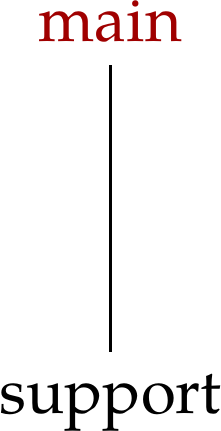
\includegraphics[height=2cm]{./figures/sec/planning/ontologygraph1.png}&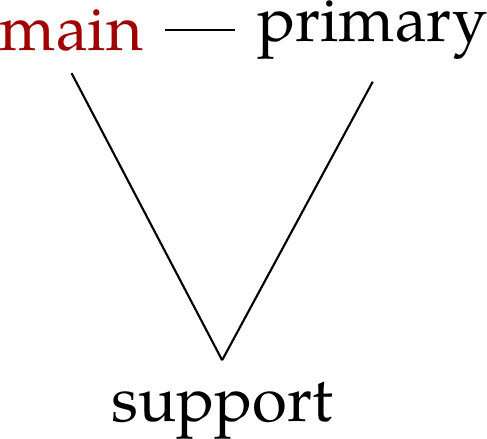
\includegraphics[height=2cm]{./figures/sec/planning/ontologygraph2.png}&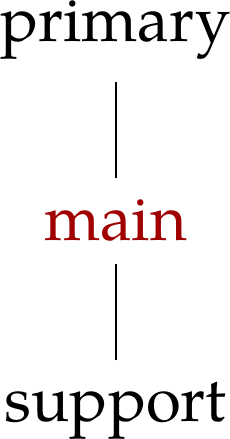
\includegraphics[height=2cm]{./figures/sec/planning/ontologygraph3.png} &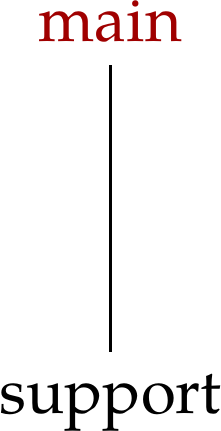
\includegraphics[height=2cm]{./figures/sec/planning/ontologygraph1.png}&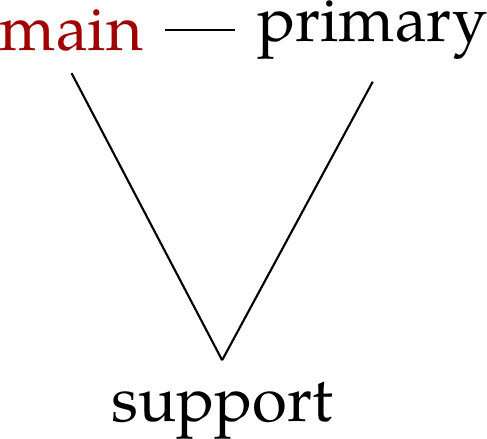
\includegraphics[height=2cm]{./figures/sec/planning/ontologygraph2.png}&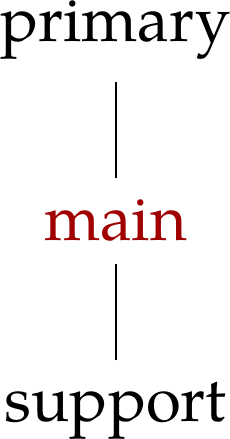
\includegraphics[height=2cm]{./figures/sec/planning/ontologygraph3.png}\\
  \midrule
  1   & Punch/hit                 & \checkmark    & \checkmark    & \checkmark  & \nmark        & \nmark        & \nmark\\
  2   & Flick                     & \checkmark    & \checkmark    & \checkmark  & \nmark        & \nmark        & \nmark\\
  3   & Poke                      & \checkmark    & \checkmark    & \checkmark  & \nmark        & \nmark        & \nmark\\
  4   & Chop                      & \checkmark    & \checkmark    & \xmark      & \nmark        & \nmark        & \nmark\\
  5   & Turn/bore                 & \checkmark    & \checkmark    & \checkmark  & \nmark        & \nmark        & \nmark\\
  6   & Cut                       & \checkmark    & \xmark        & \xmark      & \checkmark    & \checkmark    & \xmark\\
  7   & Scratch                   & \checkmark    & \checkmark    & \checkmark  & \nmark        & \nmark        & \nmark\\
  8   & Scissor-cut/pinch         & \checkmark    & \xmark        & \xmark      & \nmark        & \nmark        & \nmark\\
  9   & Squash, squeeze           & \checkmark    & \xmark        & \xmark      & \nmark        & \nmark        & \nmark\\
  10  & Draw                      & \checkmark    & \xmark        & \xmark      & \nmark        & \nmark        & \nmark\\
  11  & Push                      & \checkmark    & \checkmark    & \xmark      & \nmark        & \nmark        & \nmark\\
  12  & Stir                      & \xmark        & \checkmark    & \xmark      & \nmark        & \nmark        & \nmark\\
  13  & Knead                     & \checkmark    & \checkmark    & \xmark      & \nmark        & \nmark        & \nmark\\
  14  & Rub/massage               & \checkmark    & \xmark        & \xmark      & \nmark        & \nmark        & \nmark\\
  15  & Lever (rotate wrist y)    & \checkmark    & \checkmark    & \checkmark  & \nmark        & \nmark        & \nmark\\
  16  & Scoop                     & \checkmark    & \checkmark    & \xmark      & \nmark        & \nmark        & \nmark\\
  17  & Take Down                 & \checkmark    & \checkmark    & \xmark      & \nmark        & \nmark        & \nmark\\
  18  & Push down                 & \checkmark    & \checkmark    & \xmark      & \nmark        & \nmark        & \nmark\\
  19  & Rip off                   & \checkmark    & \xmark        & \xmark      & \nmark        & \nmark        & \nmark\\
  20  & Break off                 & \checkmark    & \xmark        & \xmark      & \nmark        & \nmark        & \nmark\\
  21  & Uncover by pick \& place  & \checkmark    & \xmark        & \xmark      & \nmark        & \nmark        & \nmark\\
  22  & Uncover by pushing        & \checkmark    & \xmark        & \xmark      & \nmark        & \nmark        & \nmark\\
  23  & Put on top                & \checkmark    & \checkmark    & \xmark      & \checkmark    & \checkmark    & \xmark\\
  24  & Push on top               & \checkmark    & \checkmark    & \xmark      & \checkmark    & \checkmark    & \xmark\\
  25  & Put over                  & \checkmark    & \checkmark    & \xmark      & \checkmark    & \xmark        & \xmark\\
  26  & Push over                 & \checkmark    & \checkmark    & \xmark      & \checkmark    & \xmark        & \xmark\\
  27  & Push apart                & \xmark        & \checkmark    & \xmark      & \checkmark    & \checkmark    & \checkmark\\
  28  & Push together             & \checkmark    & \xmark        & \xmark      & \checkmark    & \checkmark    & \checkmark\\
  29  & Push from x to y          & \checkmark    & \xmark        & \xmark      & \nmark        & \nmark        & \nmark\\
  30  & grasp                     & \checkmark    & \checkmark    & \xmark      & \nmark        & \nmark        & \nmark\\
  \bottomrule                                     
  \caption{List of preconditions for atomic actions on the \gls{ac:sec} level (action list as shown in~\cite{worgotter2013simple}). A ``\checkmark'' denotes that the structure is allowed, if the action needs to be executed; the actions marked with ``\xmark'' are not allowed; ``\nmark'' is used, where the structure is not applicable as the state of the \emph{secondary} is of no relevance. The left three columns show preconditions for the \emph{main} object. The right columns show the preconditions of the \emph{secondary} object of an action. Please note that the action's \emph{secondary} object turns into the \emph{main} object of the subgraph.}
  \label{tab:sec_usingaffordanceforplanning_preconditions}
\end{longtable}
\end{landscape}


All these approaches are problematic as it remains difficult to smooth\-ly link sensor signals (\eg from scene analysis) to symbolic action concepts and back to the signal domain to create trajectories needed by the robot's actuators.
We ask: What is needed to push (or pick, or cut, \etc) a certain object? 
Which are the general preconditions required for this regardless of the actual objects in the scene? 
And --- if those hold --- are also the specific conditions met to actually do it?


The original \gls{ac:esec} framework did not much care about objects. 
Here, a layered structure on top of the Semantic Event Chains is incorporated, which still allows affordance analysis.
This will create an object-action-linked ontology of manipulations, where these object roles define the general preconditions that need to be met to perform a certain action at all. 


In this study the robot selects one object in a scene and asks --- like a child during play --- what could I do with it? 
The framework will then analyze the situation and suggest possible manipulation actions, thereby addressing the problem of context dependent affordances.
A three-layered system is used: During the first layer \gls{ac:sec}-based relations are evaluated.
The second layer solely analyzes the topological structure of the \emph{main} object, and the third layer consists of a set of movement primitives, which are needed to execute the action.


\paragraph{Layer 1: \gls{ac:sec}-based object relations at start.} The first layer analyzes wheth\-er the first matrix of a Semantic Event Chain is fulfilled. 
If, and only if these touching relations are not violated, the action could commence. 
This is not yet sufficient to select actions.


\paragraph{Layer 2: Object Topologies.}
All actions are always performed at the \emph{main} object and this will only be possible, if the SEC-preconditions hold and if the \emph{main} object appears in the scene with certain topological connections to other objects. 
To analyze these connections, the nearest neighbors of the \emph{main} object are inspected as shown in \secref{ssec:action_methods_structuralinformation}.
Using these subgraphs, one can determine the remaining preconditions. 
For example, a tower structure around the \emph{main} object is not allowed for a pushing action as the top object could fall down.
Now, one can attach a set of allowed structures to each action.

One action may include more than one object, \eg \action{push object 1 and object 2 together}, where object 1 is treated as \emph{main} object and object 2 as \emph{secondary}.
Of course, the preconditions for the \emph{secondary} object also need checking.
A complete list of all preconditions is shown in \tabref{tab:sec_usingaffordanceforplanning_preconditions}.
The left three columns show preconditions for the \emph{main} object.
As explained above, subgraphs around the \emph{main} object are created and each subgraph is checked.
The right columns show the same for the \emph{secondary} object.
Please note that the \emph{secondary} object of the selected action becomes the \emph{main} object of the subgraph.


\paragraph{Layer 3: Movement Primitives.} The third layer consists of a set of movement primitives as described in~\cite{aeinaksoytamosiunaite2013}. 
These movement primitives are hardware dependent.
Two such commands shall be explained in more detail and serve as an example: \emph{move(object, transformation T)} and \emph{grasp(object)}.
The \emph{move(object, transformation T)} primitive sends a command to the robot to move to a pose which is determined by applying transform $T$ to the pose of $object$. 
The transformation $T$ contains a translation vector and rotation matrix.
\emph{grasp(object)} closes the fingers of the robot hand to securely grasp an object.


For example, when the robot should grasp the \emph{main} object, the \emph{move(main, T)} primitive is performed to move the robot arm end effector to a proper pose for grasping. 
The translation vector of transformation $T$ will lead the hand to the object, while the rotation part needs to be set such that the robot approaches the \emph{main} object from a proper angle.
This is necessary to avoid possible collisions with other objects near the \emph{main}.
The parameters for the transformation and an object's pose are taken from \gls{ac:esec}.


For testing the algorithm on real world robot hardware, the processing pipeline is as follows:

\begin{enumerate}
  \item One object is chosen as \emph{main}. This may happen by user input, or as the output of another, higher level algorithm. Here, a toddler playing and learning about its environment is simulated. This means a \emph{main} object is chosen randomly and the question is what one can do with it.
  \item The complete list of all considered manipulation actions, of which there are 30 (see \tabref{tab:sec_definitionofactions_actiontable}), is loaded.
  \item For all of them the first layer of the ontology is used to check wheth\-er the \emph{main} object in this scene fulfills its \gls{ac:sec} preconditions. 
  \item For those which passed the first layer successfully, all possible subgraphs around \emph{main} are computed and checked with the second layer of the ontology: The topological preconditions by which the list gets further reduced.
  \item Now one can use the third layer and extract the required action primitives from the ontology.
  \item This concludes the preparation stage and this information is sent to the execution engine.
\end{enumerate}

